\section{Finding the Right Prices}


The question remains: What is the right price? Should we average the
\(l^{(j)}_i\) somehow?

It turns out, that ensuring supply to be equal to demand
\(S=D\) leaves us with very little choice when it comes to prices anyway.
Let us see what happens for a fixed price vector. We want \(S=D\). This
obviously implies
\begin{equation}
	\label{eq: supply gdp = demand gdp}
	0 =\langle S-D,p\rangle =  \sum_{i=1}^n \langle S_i - D_i, p\rangle
\end{equation}
A market based system on the other hand ensures
\[
	0 = \langle S_i - D_i, p\rangle
	= \underbrace{\langle S_i, p\rangle}_{\text{income}}
	- \underbrace{\langle D_i,p\rangle}_{\text{expenses}}
\]
which is more than sufficient for the sums in Equation~\eqref{eq: supply gdp =
demand gdp} to be equal, but not sufficient for \(S=D\). In fact, it only
ensures that the price is orthogonal to the demand/supply mismatch \(S-D\).
If there are \(d\) products, that leaves a \(d-1\) hyperplane.

But as we will see, there are some price vectors, which do ensure \(S=D\).
We call these economic equilibria.

\begin{figure}
	\centering
	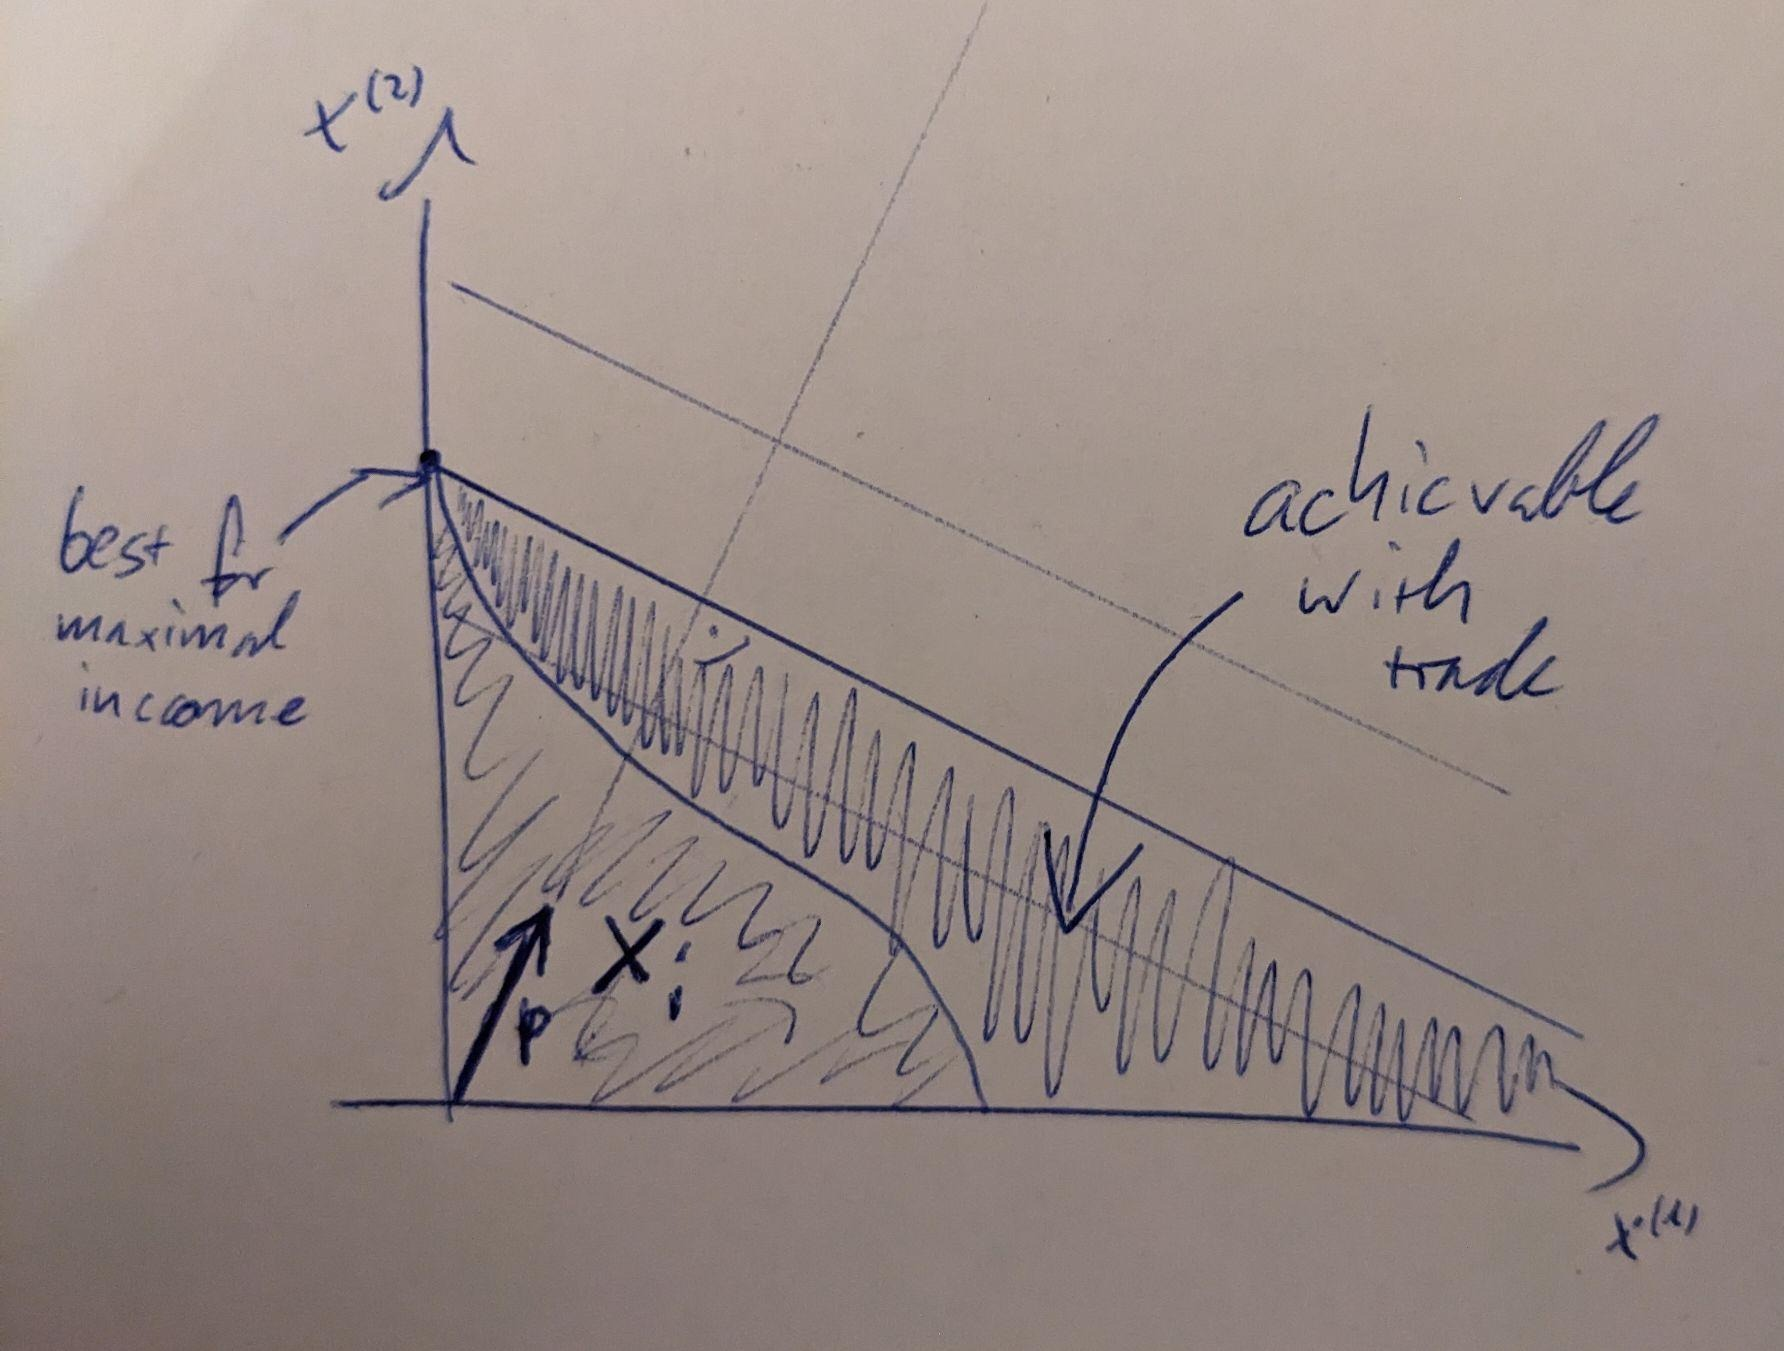
\includegraphics[width=0.7\textwidth]{images/consumption_increase_by_trade.jpeg}
	\caption{
		Product vectors on the \(d-1\) dimensional hyperplanes orthogonal to \(p\)
		cost the same amount and can therefore be exchanged (here \(d=2\), so the
		hyperplanes are lines). Trading at prices \(p\) enlarges the set of
		product vectors available for consumption for person \(i\).
	}
	\label{fig: consumption increase by trade}
\end{figure}
For a fixed price vector \(p\), let us consider the production and consumption
decision of person \(i\). As their expenses have to be smaller than their
income, it makes sense to maximize income for a given amount of labour \(L_i\).
Recall that our production options are \(X_i=X_i(L_i)\). So the maximal income
given labour \(L_i\) is
\[
	\tag{income}\label{eq: income}
	\mu(p, X_i) := \sup\{\langle p, x\rangle : x\in X_i\}.
\]
The function \(\mu(\cdot, X_i)\) in \(p\), is called the ``support function'' of
\(X_i\). It has some useful properties we will be grateful for later on. The
individual decision problem of person \(i\) therefore becomes
\begin{equation}
	\tag{IDP}
	\label{eq: individual decision problem}
	\max_{L_i, y} u(1-L_i, y) \quad\text{subject to}\quad \langle y, p\rangle \le \mu(p, X_i(L_i))
\end{equation}
In Figure~\ref{fig: consumption increase by trade} we can see, how this
constraint is always weaker than \(y\in X_i(L_i)\), which is the constraint of
self-sufficiency. I.e. we get the following lemma.

\begin{lemma}[Trade is never harmful]
\[
	\underbrace{X_i(L_i)}_{\text{own production}}
	\subseteq \quad
	\underbrace{
		\{y\in\real_{\ge 0}^\dims: \langle y, p\rangle \le \mu(p, X_i)\}
	}_{\text{consumption options with trade}}
\]
\end{lemma}
\begin{proof}
	Choose an arbitrary \(y\in X_i\), then by definition of \(\mu\)
	\[
		\langle p, y\rangle \overset{y\in X_i}\le \sup\{\langle p, x\rangle : x\in
		X_i\} \overset{\text{def.}}= \mu(p, X_i),
	\]
	\(y\) is also in the set on the right.
\end{proof}


\begin{lemma}[Income in the Pure Variable Cost Case]
	In the pure variable cost case \(L_i(x) = \langle l_i, x\rangle\), income
	can be written as
	\[
		\mu(p, X_i(L_i))
		= \overbrace{L_i}^{\text{work time}} \max_{j=1,\dots,\dims}
		\underbrace{\frac{p_j}{l_i^{(j)}}}_{=: w_i^{(j)}}
		= L_i \overbrace{\|w_i\|_\infty}^{\text{wage}},
	\]
	where \(w_i^{(j)}\) are potential wages for producing good \(j\).
\end{lemma}
\begin{proof}
	Let \(H:= \diag(l_i)\), then as \(X_i\) is compact we know the supremum is
	a maximum and
	\begin{align*}
		\mu(p, X_i)
		&= \max_{x\ge 0} \langle p, x\rangle
		\text{ s.t. } \langle x, l_i\rangle \le L_i\\
		&\overset{y=Hx}= \max_{y\ge 0} \langle p, H^{-1}y\rangle
		\text{ s.t. } \underbrace{\langle H^{-1}y, l_i\rangle}_{
			= \langle y, 1 \rangle = \|y\|_1
		} \le L_i\\
		&= L_i \underbrace{
			\max_{y\ge 0} \langle H^{-1}p, y\rangle \text{ s.t. } \|y\|_1 \le 1
		}_{
			= \|H^{-1} p\|_{\text{Op-Norm(1)}} = \|H^{-1} p \|_\infty
		}\\
		&= L_i \max_{j=1,\dots,\dims} \frac{p_j}{l_i^{(j)}},
	\end{align*}
	where we have used, that all entries of \(y\) are non-negative when
	converting to the \(1\)-norm, \(\|x\|_1 = \sum_{i=1}^\dims |x_i|\), the
	fact that the operator norm of the \(1\)-norm is the sup norm
	\(\|x\|_\infty = \sup_{i=1,\dots,\dims} |x_i|\)\fxnote{source or appendix},
	and finally positivity of entries of \(p\) and \(l_i\) again.
\end{proof}

\begin{example*}[Pure Variable Cost Case]
	The individual decision problem \eqref{eq: individual decision problem}
	therefore becomes
	\[
		\max_{L_i, y} u(1-L_i, y) \text{ s.t. } \langle p, y\rangle \le L_i \|w_i\|_\infty
	\]
	or in other words
	\[
		\max_{y} u\left(1- \frac{\langle p, y\rangle}{\|w_i\|_\infty}, y\right).
	\]
	The first order condition is therefore
	\[
		\frac{du}{dy} 
		= u_f\Bigl[
			\underbrace{\frac{u_y}{u_f}}_{\text{wtw}}
			- \overbrace{\frac{p}{\|w_i\|_\infty}}^{\text{effort required}}
		\Bigr]
		= \frac{u_f}{\|w_i\|_\infty}\Bigl[
			\underbrace{\frac{u_y}{u_f}\|w_i\|_\infty}_{\text{wtp}}
			- p
		\Bigr]
	\]
	Where the ``willingness to pay'' (wtp) is simply the willingness to work
	(wtw) scaled by person \(i\)'s wages.
	
\end{example*}


\subsection{Aggregate Production Capabilities}

The total production capabilities of a society is given by the Minkowski sum\footnote{
	The Minkowski sum of set \(A\) and \(B\) is defined as
	\[
		A + B := \{ x+y : x\in A, y\in B\}
	\]
}
of individual production capabilities
\begin{equation}
	\label{eq: tpc}\tag{TPC}
	X = \{ x_1 + \dots + x_n : x_i \in X_i\} = \sum_{i=1}^n X_i
\end{equation}

If we split the spoils of production equally between everyone, then the set of
possible consumption vectors is given by the average production capability
\begin{equation}
	\label{eq: apc}\tag{APC}
	\bar{X}_n = \tfrac1n X = \{\tfrac{x}n : x\in X\}.
\end{equation}

In a society of identical clones, this is what we would expect to happen.

\begin{lemma}[Clone Production Capabilities]
	In a society of clones, we have \(X_1=\dots = X_n\).
	to make the following two observations:
	\begin{enumerate}
		\item In general we have \(X_1\subseteq \bar{X}_n\).
		\item If we assume that \(X_1\) is convex, then
		\[
			\bar{X}_n = X_1
		\]
		\item Using only the \ref{eq: lower layer} property of \(X_1\), we get
		\[
			\bar{X}_n \to \conv(X_1),
		\]
		where \(\conv(M)\) is the convex hull\footnote{
			The convex hull is defined as the set of all convex combinations
			\[
				\conv(M)= \Bigl\{\sum_{i=1}^m \lambda_i x_i : m\in\nat,\ x_i \in M,\ \lambda_i\in[0,1],\ \sum_{i=1}\lambda_i =1\Bigr\}
			\]
		} of the set \(M\) and we define
		convergence of sets as follows: \(M_n\) converges to \(M\), if

		\begin{enumerate}
			\item\label{set-conv: seq} For all \(x\in M\) exists a sequence
			\(x_n\in M_n\) with \(x_n\to x\).

			\item\label{set-conv: incl} For all \(x\) in the interior \(M^\circ\)
			of \(M\), exists \(n_0\in\nat\) such that \(x\in M_n\) for all \(n\ge
			n_0\).
		\end{enumerate}
		The \ref{eq: lower layer} property is only needed for \ref{set-conv:
		incl}.
	\end{enumerate}
\end{lemma}

\begin{proof}
\begin{enumerate}
	\item For \(X_1 \subseteq \bar{X}_n\), we take \(x\in X_1\) and
	observe that if we pick 
	\[
		x_1=\dots=x_n=x
	\]
	in the Minkowski sum we obtain \(n x \in X\). So we have
	\(x\in\bar{X}_n\).
	

	\item
	Equality in the convex case is almost trivial as well. Let \(x\in
	\bar{X}_n\), then there exist \(x_1,\dots,x_n \in X_1\) such that \[
		x = \frac1n \sum_{i=1}^n x_i = \sum_{i=1}^n \frac1n x_i
		\overset{\text{convex}}\in X_1.
	\]

	\item
	\begin{enumerate}
		\item Pick \(x\in \conv(X_1)\). Since it is in the convex hull,
		there exist \(\lambda_1,\dots,\lambda_m\) summing to unity, \(x_i\in X_1\)
		with
		\[
			x = \sum_{i=1}^m \lambda_i x_i.
		\]
		We set the number of clones producing \(x_i\) to the largest integer smaller
		\(n\lambda_i\)
		\[
			k_i^{(n)} := \lfloor n\lambda_i \rfloor.
		\]
		This is possible due to	
		\[
			\sum_{i=1}^m k_i^{(n)} \le n \sum_{i=1} \lambda_i = n.
		\]
		This results in
		\[
			x^{(n)}:= \frac1n\sum_{i=1}^m k_i x_i \in \bar{X}_n.
		\]
		Due to \(\frac{k_i^{(n)}}{n}\to \lambda_i\), we can conclude \(x^{(n)}\to
		x\).
		
		\item
		Pick any \(x=(x^{(1)},\dots,x^{(\dims)})\in\conv(X_1)^\circ\). Since it is
		in the interior, there exists \(\epsilon>0\) such that
		\[
			x_{+\epsilon}
			:= (x^{(1)}+\epsilon, \dots, x^{(\dims)}+\epsilon) \in \conv(X_1)^\circ.
		\]
		By \ref{set-conv: seq} we know there exists a sequence
		\(x_n\in\bar{X}_n\) with \(x_n\to x_{+\epsilon}\), and therefore there exists
		\(n_0\in\nat\) such that for all \(n\ge n_0\), \(x_n\) is included in the
		\(\epsilon\) ball induced by the sup-norm around \(x_{+\epsilon}\). But this
		implies \(x^{(i)} \le x^{(i)}_n\) for all \(n\ge n_0\). As the \ref{eq: lower
		layer} property easily translates\footnote{
			the lower layer property essentially allows us to throw away surplus. It
			is intuitive that we can do that with the total output as well. To show
			this mathematically we only need to distribute this ``throwing away''
			action among the producers of the product we want to throw away.
		} to the
		Minkowski sum and the average production capabilities \(\bar{X}_n\), we
		conclude \(x\in\bar{X}_n\) for all \(n\ge n_0\).
		\qedhere
	\end{enumerate}
\end{enumerate}
\end{proof}

In general, the production sets \(X_i\) are obviously not equal. But assuming
they are drawn from some sort of probability distribution, it seems plausible
that \(\bar{X}_n\) would still converge to a convex set. But defining a
probability distribution over the sets with the \ref{eq: lower layer} property,
is not trivial to do. Later we will consider the special case of an
extended pure variable cost case (with setup costs), where the costs are random
variables.\fxnote{add reference}

\begin{lemma}[Production Frontier]
	If \(X\) is a compact, convex \ref{eq: lower
	layer}, then for any \(x\in \partial X\), there exists
	\(p\neq 0\) such that
	\begin{equation}
		\label{eq: prod frontier p}
		x \in \argmax_{y\in X} \langle p, y\rangle %= \nabla_p \mu(p, X)
	\end{equation}
	and therefore
	\[
		\mu(p, X) = \langle p, x\rangle.
	\]
	If additionally \(x\in\real_{>0}^\dims\), then necessarily \(p\in\real_{\ge
	0}^\dims\) if \(p\) satisfies \eqref{eq: prod frontier p}.
\end{lemma}
\begin{proof}
	Let \(x\in \partial X\), define \(A:=X^\circ\) and \(B:=\{x\}\). Then \(A\)
	is open; \(A\) and \(B\) are disjoint, nonempty
	convex subsets of \(\real^\dims\). So by the hyperplane separation theorem
	there exists
	\(0\neq p\in\real^\dims\) and \(c\in\real\) with
	\[
		\forall y\in A : \langle y, p\rangle < c
		\qquad\text{and}\qquad
		\langle x, p\rangle \ge c.
	\]
	Due to continuity of the scalar product we also have \(\langle y, p\rangle
	\le c\) for all \(y\in X\). Since \(x\in X\) this implies
	\begin{equation}
		\label{eq: x is max w.r.t. p}
		\langle y, p\rangle \le c = \langle x, p\rangle \quad \forall y\in X
	\end{equation}
	Therefore \(x\in\argmax_{y\in X} \langle p, y\rangle\) and \(\mu(p, X) =
	\langle x, p\rangle\).

	Let us now consider \(x=(x^{(1)},\dots,x^{(\dims)})\in\real_{>0}^\dims\).
	To arrive at a contradiction, we assume \(p_i < 0\). Since \(x^{(i)}>0\) and
	\(X\) is a \ref{eq: lower layer}, we can replace the entry \(x^{(i)}\) with
	\(0\) to obtain \(\tilde{x}\in X\). Then
	\[
		\langle \tilde{x}, p\rangle
		= \sum_{\substack{j=1\\i\neq j}} x^{(j)} p_j
		> \underbrace{x^{(i)}}_{>0}\underbrace{p_i}_{<0}
		+ \sum_{\substack{j=1\\i\neq j}} x^{(j)} p_j
		= \langle x, p\rangle,
	\]
	which is a contradiction to \eqref{eq: x is max w.r.t. p}.
\end{proof}


\begin{example*}[Pure Variable Cost]

\end{example*}

\begin{figure}
	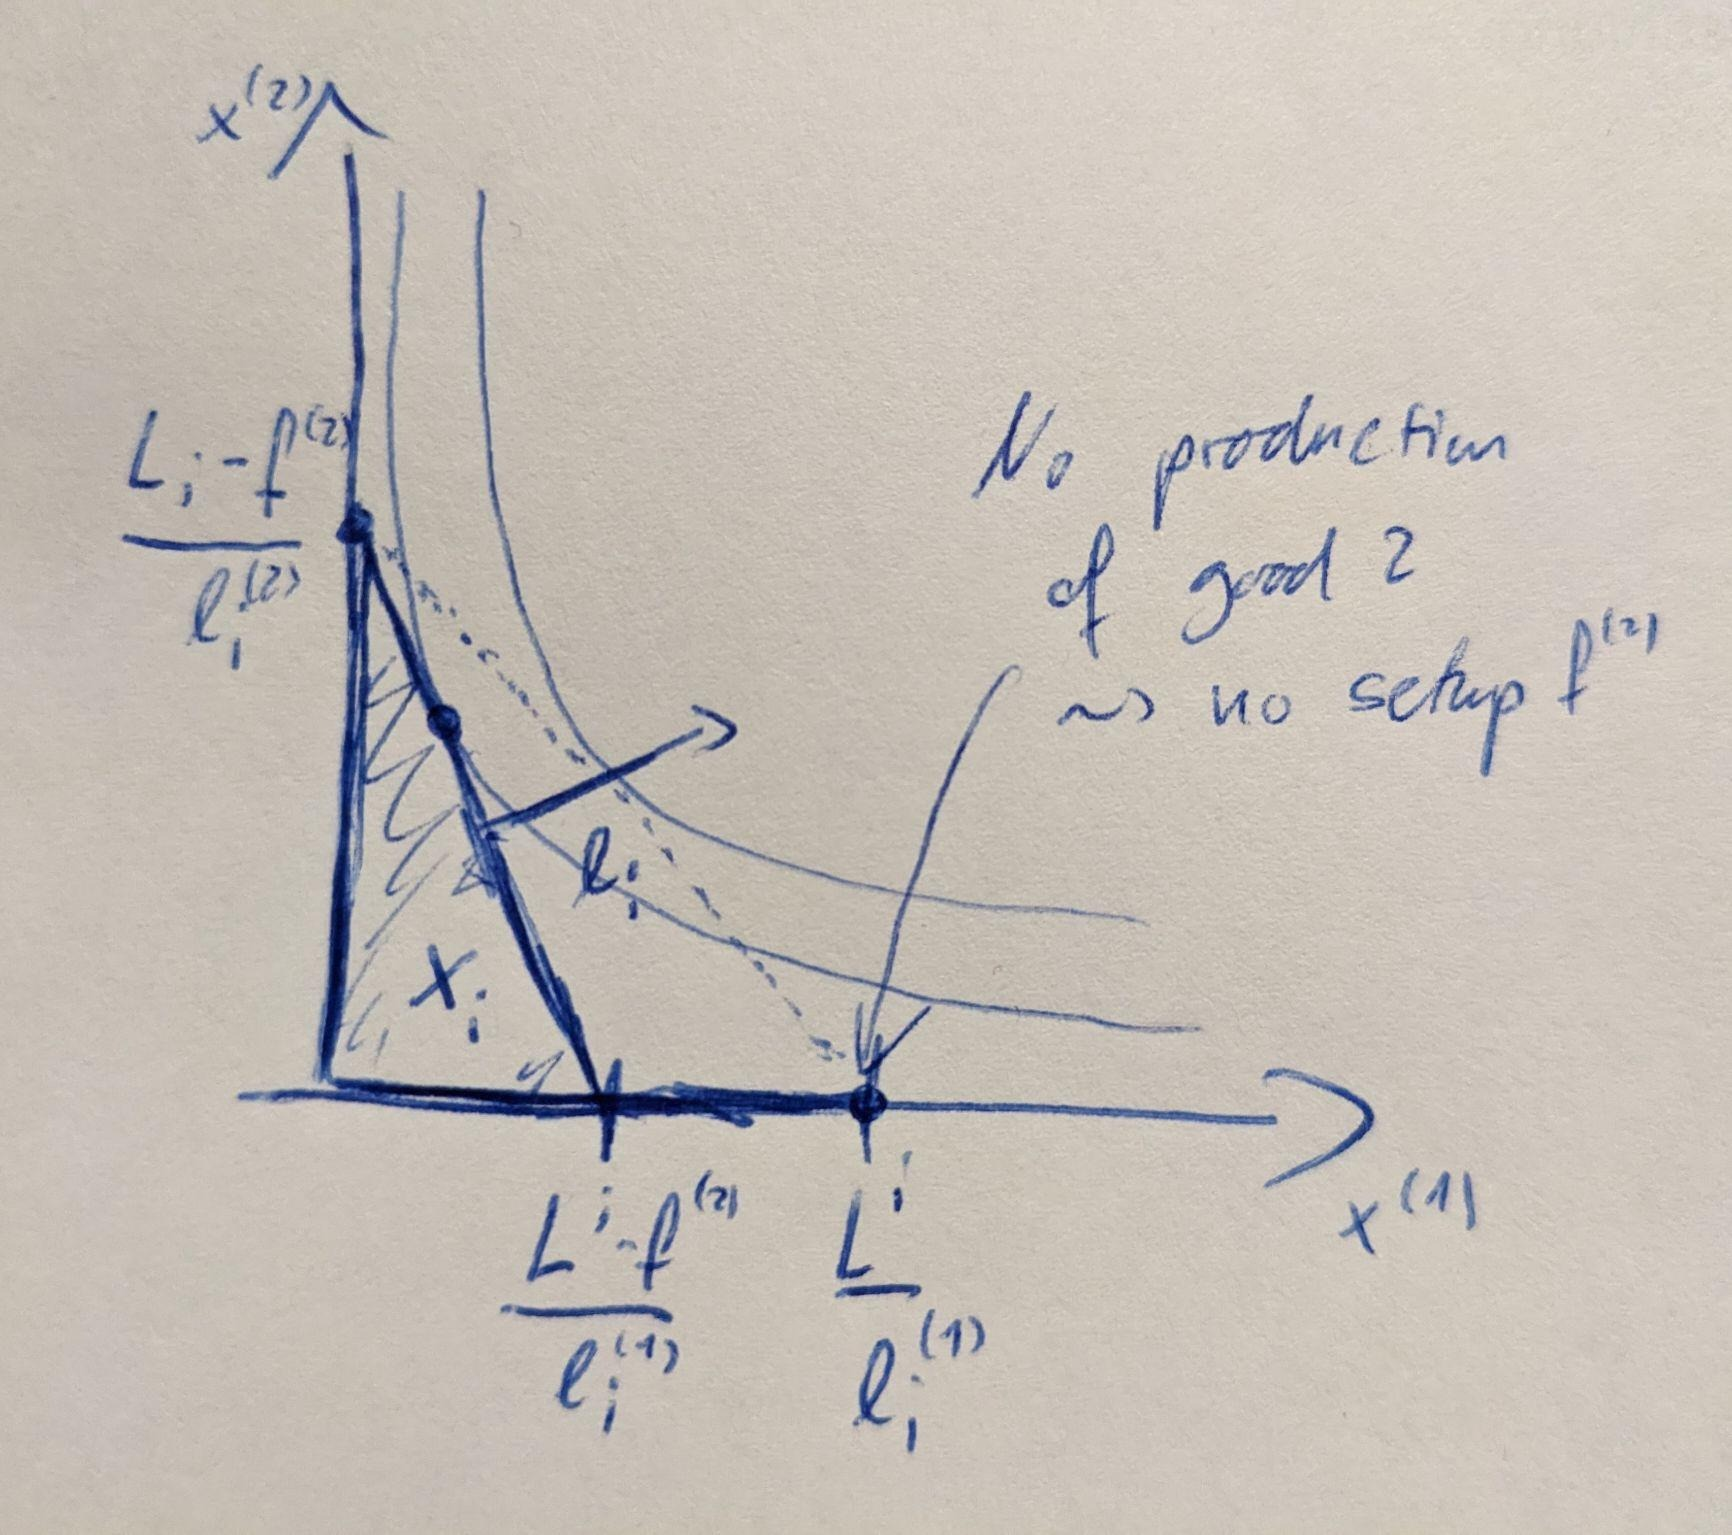
\includegraphics[width=0.58\textwidth]{images/hermit-decision-setup-cost.jpeg}
	\caption{
	fixed set-up time \(f^{(2)}\) for the production of good \(2\). This allows
	for more production of good \(1\) if \(x^{(2)}=0\). The dotted line
	represents the production frontier in the ``cloned hermit economy''.}
\end{figure}

\subsection{Supply and Demand}

Before we move on, let us quickly define supply and demand. The demand of
individual \(i\) is given by
\[
	D_i(p) := \{
		y : (L,y)
		\text{ is a solution to \eqref{eq: individual decision problem}}
	\}.
\]
Notice that it is a set, since there might be multiple solutions. The same is
true for the supply of individual \(i\)
\[
	S_i(p) := \argmax_{x\in X_i} \langle p, x\rangle 
	\overset{(*)}= \nabla_p \mu(p, X_i).
\]
Where \((*)\) is a property of the support function \(\mu(\cdot,
X_i)\)\fxnote{source or explanation}.
We can then define total demand and supply
\[
	D(p) := \sum_{i=1}^n D_i(p),
	\qquad
	S(p) := \sum_{i=1}^n S_i(p),
\]
where the sums are Minkowski sums.
And \(p^*\) is a market equilibrium, if
\[
	S(p^*)\cap D(p^*)\neq\emptyset.
\]
If \(S(p^*)\) and \(D(p^*)\) only contain a single element, one may write
\(S(p^*)=D(p^*)\).